%% LyX 2.1.4 created this file.  For more info, see http://www.lyx.org/.
%% Do not edit unless you really know what you are doing.
\documentclass{article}
\usepackage[latin9]{inputenc}
\usepackage[a4paper]{geometry}
\geometry{verbose,lmargin=2.59cm}
\usepackage{amsmath}
\usepackage{amssymb}
\usepackage{graphicx}

\makeatletter
%%%%%%%%%%%%%%%%%%%%%%%%%%%%%% User specified LaTeX commands.
%\usepackage{amsrefs}
\usepackage{amsthm}
\usepackage{graphicx}


% \DeclareMathOperator{\unit}{u} \DeclareMathOperator{\comb}{comb}
\DeclareMathOperator{\tri}{tri} \DeclareMathOperator{\rect}{rect}
\DeclareMathOperator{\sgn}{sgn} \DeclareMathOperator{\ramp}{ramp}
\DeclareMathOperator{\sinc}{sinc}


\date{ }

\makeatother

\begin{document}

\title{Bijzondere functies}
\maketitle
\begin{itemize}
\item Wat is de grafiek van de absolute waarde functies?
\item Wat betekent de functie sgn(x)?
\end{itemize}

\section{De absolute waarde}

\noindent In Module 1: Elementaire vaardigheden A heb je reeds de
definitie gezien van de absolute waarde:

${\displaystyle \left|x\right|=\begin{cases}
-x & \textrm{als}\:x<0\\
x & \textrm{als}\:x\geq0
\end{cases}}$

\medskip{}


\noindent en de bijhorende grafiek:

\noindent 
\begin{figure}[h]
\centering{}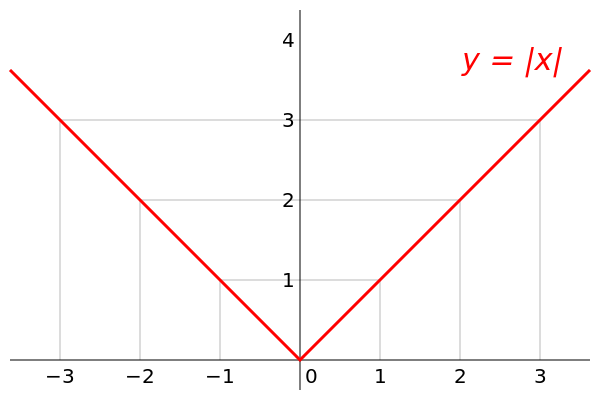
\includegraphics[height=5cm]{figures/Absolute_value_svg} 
\end{figure}


\noindent We hebben er toen ook op gewezen dat je voorzichtig moet
zijn met formules van het type $\sqrt{x^{2}}$.

\noindent Passen we dit toe op een functie die horizontaal verschoven
is: ${\displaystyle y=\sqrt{(x-1)^{2}}=\left|x-1\right|}$.

\noindent Als deze functie zou gegeven zijn als de veelterm ${\displaystyle x^{2}-2x+1}$,
dan loont het dus de moeite om dit te herschrijven als een volledig
kwadraat: ${\displaystyle x^{2}-2x+1=\left(x-1\right)^{2}}$.


\section{De signum functie}

De sign of signum functie $\textrm{sgn}(x)$ is een eenvoudige wiskundige
functie, die eigenlijk het teken van het argument aangeeft:

${\displaystyle \textrm{sgn}(x)=\begin{cases}
-1 & \textrm{als}\:x<0\\
0 & \textrm{\textrm{als}}\:x=0\\
+1 & \textrm{\textrm{als}}\:x>0
\end{cases}}$

\medskip{}


\noindent De grafiek van de signum functie:

\noindent 
\begin{figure}[h]
\centering{}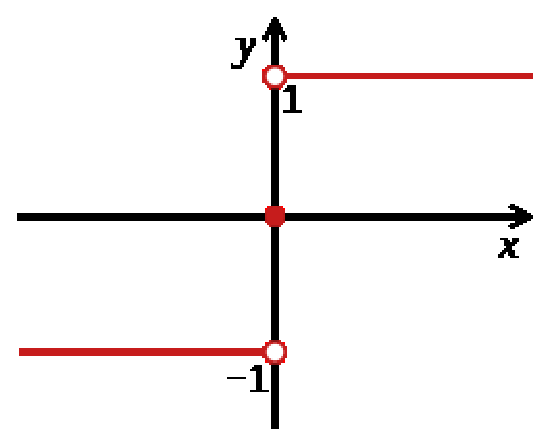
\includegraphics[height=5cm]{figures/Signum_function_svg} 
\end{figure}

\end{document}
